\section{Quantitative Study: Europe and United States}
\label{res}
In this section, we discuss the results from our quantitative survey. We extended our questionnaire from our previous work \cite{BatesESP} and contacted sixteen SCs in the European region.  Appendix \ref{appendixA} provides an overview of the questionnaire. The detailed definitions for each of the demand management approaches and strategies can be found in our previous work \cite{BatesESP}. Nine out of the sixteen European SCs that we contacted responded to the questionnaire. All except one of these sites were in Top 50 supercomputers in the world \cite{Top500}. 


\begin{figure}[ht!]
\begin{center}
\frame{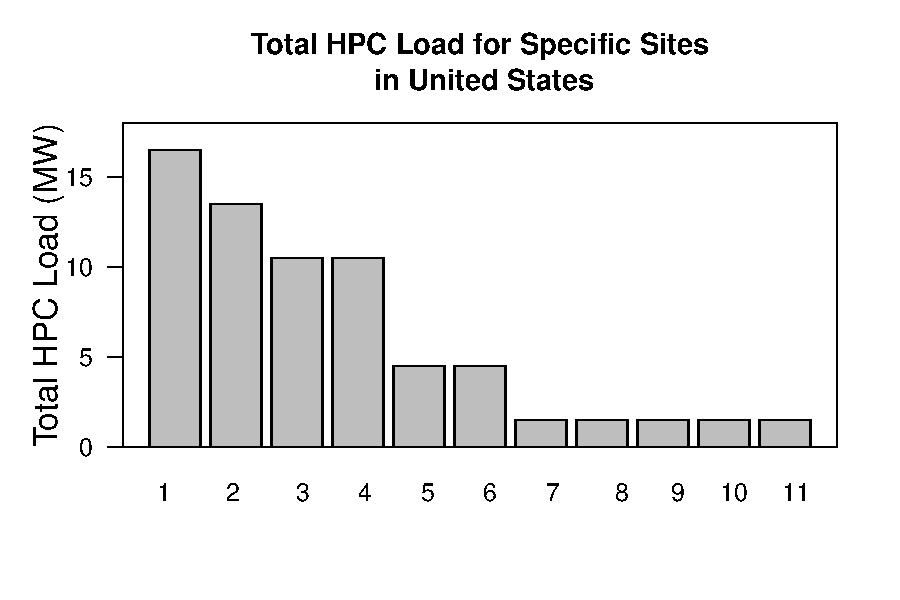
\includegraphics[scale=0.58]{figs/loadgraphUS.pdf}}
\caption{Total Load at at SCs in United States}
\label{fig:USload}
\vspace{0.9cm}
\frame{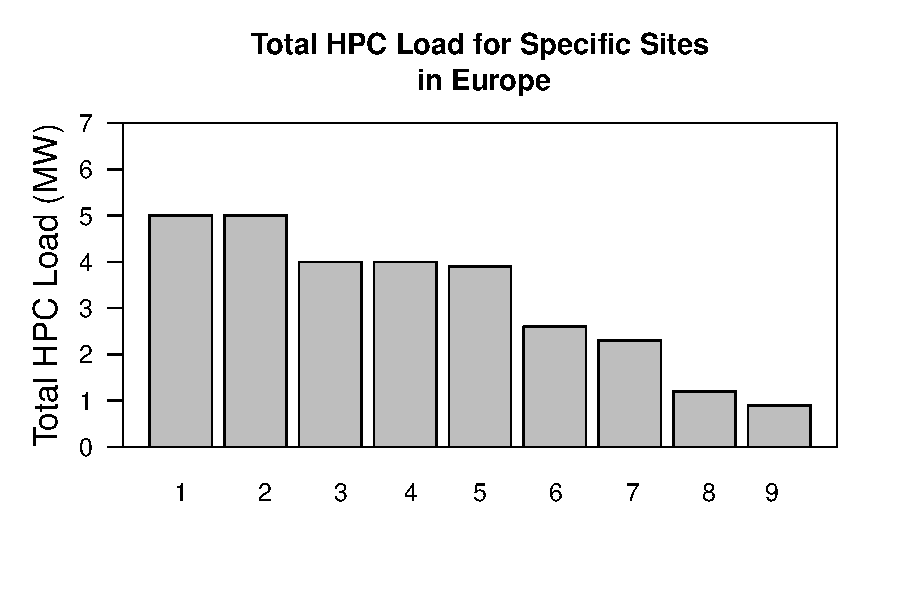
\includegraphics[scale=0.58]{figs/loadgraphEU.pdf}}
\caption{Total Load at at SCs in Europe}
\label{fig:EUload}
\end{center}
\end{figure}

Figures \ref{fig:USload} and \ref{fig:EUload} depict the total load in megawatts for each of the respondents in the United States and in Europe. Most supercomputing sites have a total load of under 5 MW (sixteen out of twenty). Four of the surveyed supercomputing sites had a total load of over 10 MW. 

\begin{figure}[ht!]
\begin{center}
\frame{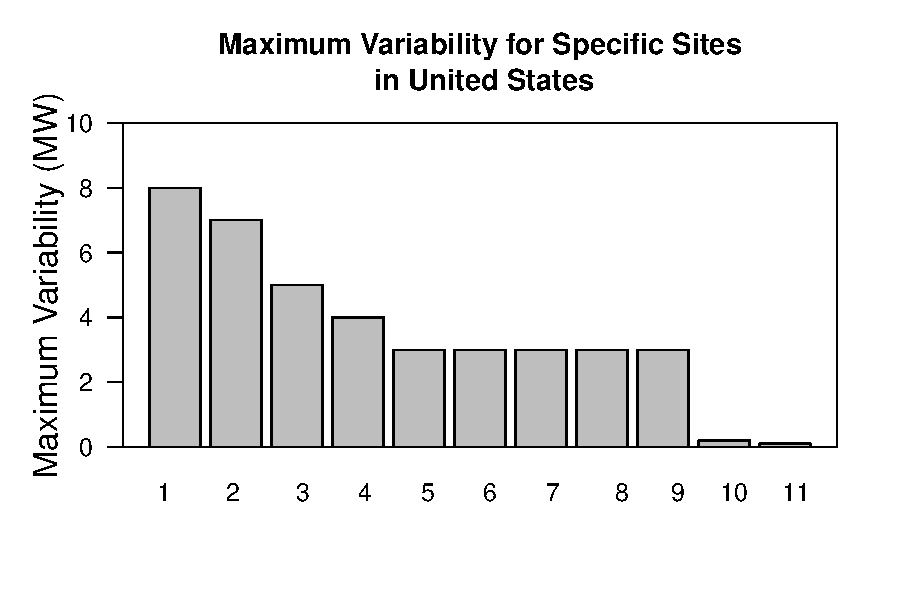
\includegraphics[scale=0.58]{figs/vargraphUS.pdf}}
\caption{Maximum Variability at at SCs in United States}
\label{fig:USvar}
\vspace{0.9cm}
\frame{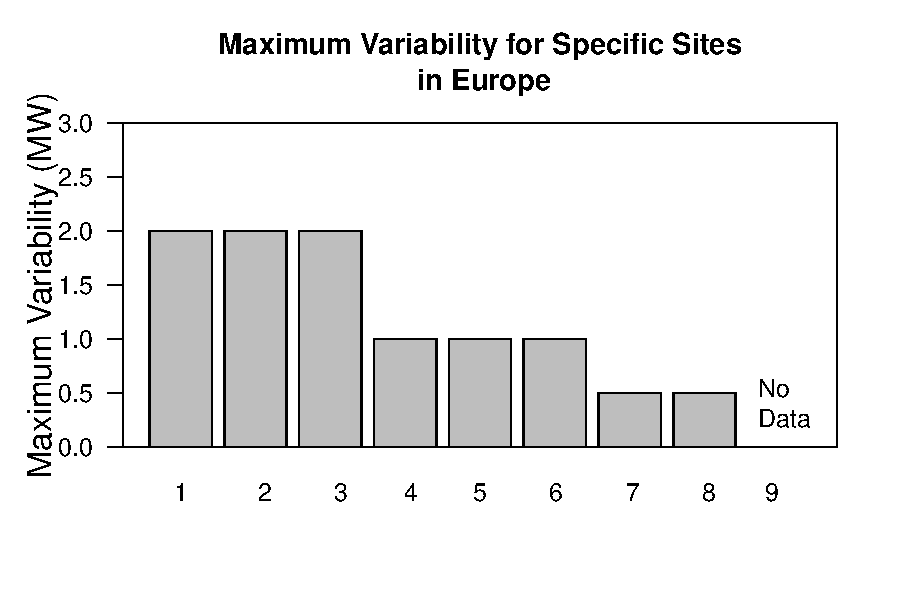
\includegraphics[scale=0.58]{figs/vargraphEU.pdf}}
\caption{Maximum Variability at at SCs in Europe}
\label{fig:EUvar}
\end{center}
\end{figure}

Both United States and Europe had power swings and fluctuations of a few megawatts. In our questionnaire, we asked respondents to report the maximum variability that they have experienced in their SCs. The results of these for United States as well as Europe are shown in Figures \ref{fig:USvar} and \ref{fig:EUvar} respectively. In the United States, three of the eleven sites surveyed had maximum variability of over 5 MW. For our United States respondents, the minimal option for reporting this was ``Less than 3 MW'', because of which we could not capture less intense power swings. In the European survey, we allowed the respondents to provide a more accurate value, and as shown in Figure \ref{fig:EUvar}, we observed power swings in the range of half a megawatt to about 2 MW. Almost all of the respondents reported that this variability is due to maintenance cycles, and that it can be scheduled \emph{day-ahead} if necessary.

In terms of demand management strategies, the survey indicated that there is moderate interest in grid integration strategies such as coarse- and fine- grained power management or temperature control in the United States, and low interest for the same in Europe. From the point of view of SCs, strategies such as cutting jobs or load migration have little or no interest. 

From our questionnaire, we also concluded that neither European nor the United States sites are engaged with peak shedding, peak shifting or dynamic pricing programs at present. More sites in the United States have communicated with their ESPs regarding these programs. While both European and United States SCs are interested in dynamic pricing, there is mixed interest in peak shedding and peak shifting. The European sites are more interested in peak shedding than peak shifting, but the United States sites are more interested in peak shifting. Both European and US sites are interested in discussing renewables with their ESPs, but there is little interest in communicating with regards to the other possible methods.

\begin{table}[h]
\begin{center}
\begin{tabular}{|l|c|c|c|c|}
\hline
\multicolumn{5}{|p{.72\textwidth}|}{\emph{Ques:} Please evaluate as high, medium or low the following motivations for your site's interest in pursuing a stronger relationship with your electricity service provider}\\
\hline
& Low & Medium & High & Rating Count \\
\hline
Economically justified & 14.3\% (1) & 28.6\% (2) & 57.1\% (4) & 7 \\
\hline
Good citizen & 14.3\% (1) & 71.4\% (5) & 14.3\% (1) & 7 \\
\hline
Adverse consequences & 66.7\% (4) & 16.7\% (1) & 16.7\% (1) & 6 \\
\hline
Government regulation & 71.4\% (5) & 28.6\% (2) & 0.0\% (0) & 7 \\
\hline
\end{tabular}
\end{center}
\caption{Motivation for communicating with ESP (European Respondents)}
\label{fig:table2}
\end{table}

We also asked our European respondents to indicate what might motivate them to communicate with their ESPs. The results are shown in Table \ref{fig:table2}. As can be noted from this table, the main motivators are the financial incentives and the desire to be ``good citizens.'' Thus, SC motivations are driven by market-based mechanisms that justify economics and social-responsibility, even under the absence of regulatory support.

\begin{table}[h]
\begin{center}
\begin{tabular}{|p{0.265\linewidth}|p{0.265\linewidth}|p{0.265\linewidth}|}
\hline
\textbf{Program} & \textbf{Europe} & \textbf{United States}\\
\hline
Peak Shedding & 1 & 6\\
\hline
Peak Shifting & 0 & 4\\
\hline
Dynamic Pricing & 0 & 5\\
\hline
\end{tabular}
\end{center}
\caption{Communications with ESPs regarding available programs}
\label{fig:table3}
\end{table}
We noted that none of the European SCs communicated about grid integration potential, demand management and available flexibility with their associated ESPs. Additionally, there was little interest in a tighter integration with the ESPs. In general, the SCs in the United States seem to have a closer relationship with their ESPs than the ones in Europe. This can also be verified from Table \ref{fig:table3}, which shows that only 1 of the 9 respondents in Europe have had a discussion with their ESP. 

\subsection{Comments from Survey Respondents}
\label{comm}
From the comments section in our questionnaire, we noted that all SCs are already using \emph{demand forecasting} to communicate their upcoming demands and maintenance cycle schedules with their ESPs. For example, one comment was ``We project hourly average power at least a day in advance, within +/- 1MW''. Another interesting comment was ``We've to ensure that our power load neither over- nor under-shoots the contracted power band. In any cases of foreseen power abnormalities we've to inform our grid provider at least two days ahead of schedule.''

One of the SCs mentioned that they could not provide the forecast that was being asked by their ESP. More specifically, their comment indicated that their ESP asked for ``multi-year forecast of energy requirements, additional detailed forecasting and ultimately real time data, and power projections, hour by hour, for at least a day in advance.''

When it came to ESP programs, the United States SCs showed more interest. ``Our site generates 30-35 MW of power yet still imports 5-10 MW. As a large generation source the utility providers see the campus as a highly attractive partner for offloading grid stress. automatic load shedding is being explored/deployed today,'' one of the SCs noted. Another comment was ``[We are] working on load sharing of data with utility to provide better scheduling tools and address potential grid changes.'' One of the SCs mentioned that they demonstrated that peak shedding and shifting was possible, but not deployed due to its impact on HPC productivity. 

The European SCs, on the other hand, did not have much knowledge about ESP programs. Some of the responses were ``There are not so many related options and features offered by providers. We are open to further and pro-active efforts as long as providers have other kinds of programs to propose'' and ``With many of your questions I am wondering about the kind of contracts other centers might have and about the quality of some electricity providers.''

The comments also indicated that the SCs in United States are investigating the impact of power fluctuations on the electrical grid. ``[We are] working directly with provider to ensure that the effects of large load swings are understood. Have funded a simulation that accounts for all loads.'' and ``Our provider has no problem with our load swings. They indicate no concern with our next system either, but we are still looking into possible options in case there actually is a problem.'' were some of the interesting responses.
